\section{Struktura aplikacije}

Ova aplikacija napravljena je pomoću HTML-a, CSS-a i JavaScript-a, a sastoji se od sljedećih dijelova: jedne HTML datoteke, jedne CSS datoteke, dvije JavaScript datoteke, jedne json datoteke i jedne slike koja prikazuje lopticu na ploči za igru.  Za izradu sučelja korišten je HTML u datoteci index.html, a za stil korisničkog sučelja korišten je CSS u datoteci nim.css. Glavna logika programa napisana je pomoću jezika JavaScript, u datotekama game.js i index.js. Baza podataka je datoteka users.json u kojoj su pohranjeni podaci o korisnicima i o njihovim igrama.

\begin{figure}[H]
\centering
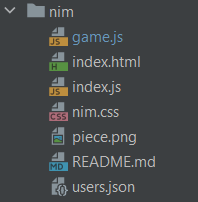
\includegraphics[]{slike-kod/Slika1.png}
\caption{Prikaz strukture koda aplikacije.}
\label{}
\end{figure}

Datoteka index.js sastoji se od tri funkcije: processPostRequest(), checkCredentials() i createServer(), koje služe za provjeru korisničkih podataka, obradu POST zahtjeva i kreiranje servera za pokretanje aplikacije.

Datoteka game.js prikazuje cjelokupnu logiku igre, a sastoji se od 15 funkcija gdje svaka funkcija ima svoju svrhu u samom programu. Funkcije koje se koriste u ovoj datoteci su:


\begin{itemize} 
\item showFrontPage() – prikaz početne stranice
\item showGameForm() -  prikaz stranice s postavkama igre
\item showRanks() – prikaz top liste najboljih igrača
\item showRules() – prikaz pravila igre
\item showGameDiv() – prikaz stranice sa igrom 
\item resetGameDiv() – uklanja stranicu s igrom
\item playGame() – inicijalizacija nove igre
\item restartGame() – ponovno pokretanje nove igre
\item login() – prijava korisnika u svoj profil
\item logout() – izlazak korisnika iz svog profila
\item leaveGame() – izlazak iz igre
\item Board() – prikaz ploče za igru
\item NimGame() – stvaranje nove igre
\item Piece() – stvaranje loptice na ploči za igru
\item PC() – određivanje poteza računala
\end{itemize}



\section{Funkcionalnosti aplikacije}



Funkcija checkCredentials() kao parametre prima korisničko ime i lozinku korisnika. Na početku pomoću funkcije createHash kreira hash lozinke korisnika. Ako to korisničko ime ne postoji u datoteci users.json, onda ga zajedno s tim hashom ubacuje u datoteku users.json, inače javlja grešku da je upisana lozinka pogrešna.  

Funkcija processPostRequest() kao parametre prima varijable zahtjeva i odgovora. Ona obrađuje POST zahtjeve ovisno o rezultatu poziva funkcije checkCredentials(). Ako je rezultat poziva funkcije jednak 2, vraća status 500, što označava grešku, a ako je rezultat poziva jednak 1 vraća status 400 s porukom da je korisnik registriran sa drugom lozinkom. U protivnom nema greške i vraća status 200. Na kraju datoteke pomoću funkcije createServer kreira se server na linku https://nim-projekt.onrender.com pomoću kojega se pokreće cijeli program.


\begin{figure}[H]
\centering
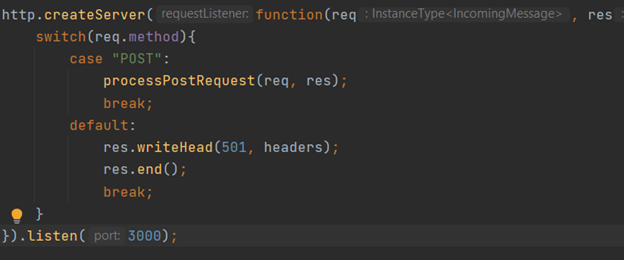
\includegraphics[width=14cm]{slike-kod/Slika2.png}
\caption{Prikaz koda funkcije createServer().}
\label{}
\end{figure}






Na početku datoteke game.js definiraju se sve varijable potrebne za pisanje programskog koda datoteke. Funkcija showFrontPage() prikazuje početnu stranicu i miče sve ostale elemente. Funkcija showGameForm() također miče sve ostale elemente, ali i ako igra još traje prikazuje ploču za igru i loptice. Također miče i formu u kojoj korisnik upisuje postavke igre. Ako korisnik nije ulogiran prikazuje formu za logiranje, a u suprotnom prikazuje formu za prikaz postavki igre. Ako upisana lozinka nije valjana prikazuje upozorenje o pogrešnoj lozinki, a isto to čini i za krivi upis veličine stupaca za igru.


\begin{figure}[H]
\centering
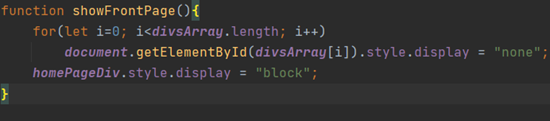
\includegraphics[width=14cm]{slike-kod/Slika3.png}
\caption{Prikaz koda funkcije showFrontPage().}
\label{}
\end{figure}

Funkcija showRanks() prikazuje top listu najboljih igrača. U tablici top lista nalaze se: korisničko ime igrača, ukupan broj njegovih igara, broj pobjeda, broj poraza i omjer njegovih pobjeda i poraza, a svi ti podaci upisuju se u users.json datoteku pomoću koje se ti podaci prikazuju korisniku. Tablica je sortirana prema omjeru pobjeda i poraza tako što je igrač sa najboljim omjerom na vrhu tablice. Funkcija showRules() prikazuje pravila igre nakon što korisnik klikne gumb za prikaz pravila igre, a s druge strane funkcije showGameDiv() i resetGameDiv() prikazuju i miču ploču s lopticama. 


\begin{figure}[H]
\centering
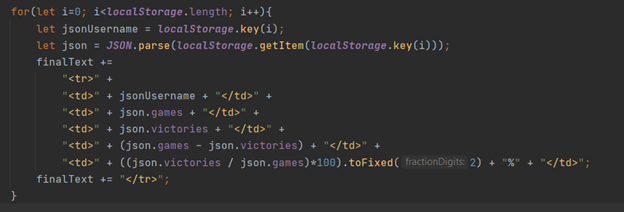
\includegraphics[width=14cm]{slike-kod/Slika4.png}
\caption{Prikaz tablice top lista iz funkcije showRanks().}
\label{}
\end{figure}


\begin{figure}[H]
\centering

\includegraphics[width=14cm]{slike-kod/Slika5.png}
\caption{Prikaz koda funkcija showRules(), showGameDiv() i resetGameDiv().}
\label{}
\end{figure}





Funkcija playGame() pomoću odabranih vrijednosti korisnika o veličini polja i igraču s prvim potezom inicijalizira novu igru, a prije toga provjerava je li upisana vrijednost veličine polja ispravna. Funkcija restartGame() samo ponovno poziva prethodno navedenu funkciju. Pomoću funkcije login() POST zahtjevom šalje se korisničko ime i lozinka igrača u datoteku users.json gdje se vodi evidencija o svim njegovim igrama, što se prikazuje u tablici igrača. Također, korisničko ime prikazuje se u gornjem desnom dijelu ekrana kako bi igrač mogao znati da je ulogiran u aplikaciju. Ako se igrač odluči izaći iz profila dok traje igra dobiva upozorenje da se to ne dozvoljava dok igra još traje, nego mu se to dozvoljava tek kada već započeta igra završi pa se prikazuje početna stranica. Također, kada igrač odluči izaći iz igre, ali ostati u svom profilu prikazuje mu se poruka o porazu i nudi se pokretanje nove igre. 



\begin{figure}[H]
\centering
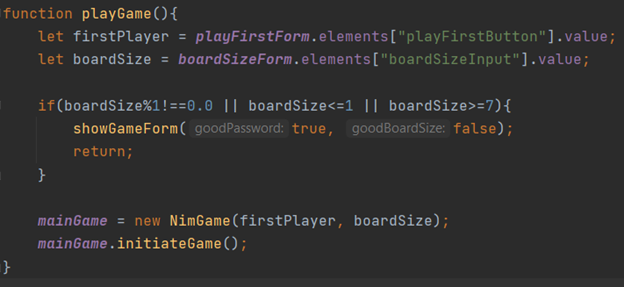
\includegraphics[width=14cm]{slike-kod/Slika6.png}
\caption{Prikaz koda funkcije playGame().}
\label{}
\end{figure}


\begin{figure}[H]
\centering

\includegraphics[width=14cm]{slike-kod/Slika7.png}
\caption{Prikaz koda funkcije login().}
\label{}
\end{figure}

\begin{figure}[H]
\centering

\includegraphics[width=14cm]{slike-kod/Slika8.png}
\caption{Prikaz koda funkcije logout().}
\label{}
\end{figure}


Ploča za igru izgrađena je od loptica koje su poredane uzlazno po stupcima tako što je u prvom stupcu jedna loptica, a svakim stupcem broj loptica se povećava za jednu, sve dok ne dođe do maksimalne razine koju je odredio korisnik u svojim početnim postavkama igre. Funkcija NimGame() inicijalizira novu igru tako što postavlja prvog igrača na potezu i kreira novu ploču za igru. Također, postavlja i poruku koji je igrač trenutno na potezu, koja se izmjenjuje svakim potezom, te oznaku da je igra u tijeku kako igrač ne bi mogao izaći iz svog profila tijekom igre.


\begin{figure}[H]
\centering
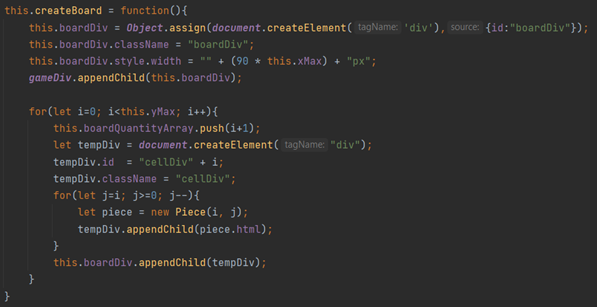
\includegraphics[width=14cm]{slike-kod/Slika9.png}
\caption{Prikaz koda za stvaranje ploče za igru.}
\label{}
\end{figure}


\begin{figure}[H]
\centering
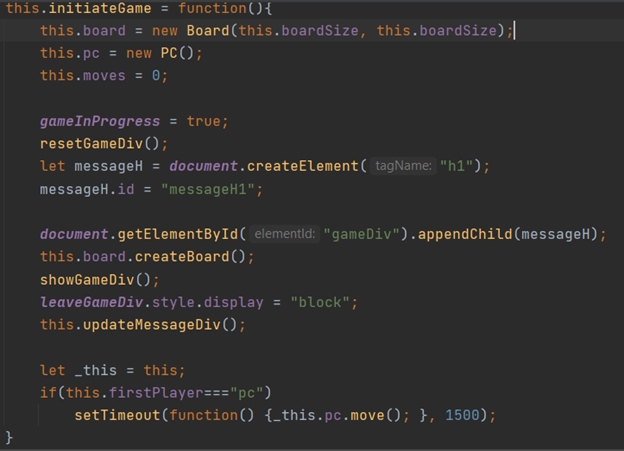
\includegraphics[width=14cm]{slike-kod/Slika10.png}
\caption{Prikaz koda za inicijalizaciju nove igre.}
\label{}
\end{figure}


 Klikom na lopticu ona se miče iz igre, a ako je to zadnja loptica na ploči, označava se kraj igre sa odgovarajućom porukom o pobjedniku, inače se provjerava koji je igrač bio na potezu i dozvoljava se drugom igraču da je na redu. Kada je igra gotova, u datoteku users.json igraču se dodaje nova igra i upisuje se je li pobijedio ili izgubio igru pa se sukladno tome računa i novi omjer pobjeda u igri. Korisnik tada može odlučiti igrati s istim ili drugačijim postavkama, a može i izaći iz profila i prestati igrati. Odlukom o izlasku iz igre dok igra traje također se u datoteku users.json dodaje nova igra i upisuje se da je korisnik poražen.

 


Glavni algoritam ovog programa je određivanje kakav će potez odigrati računalo i koje će loptice i u kojem stupcu ukloniti. Naime, u igri Nim s dva igrača, ako imamo n stupaca loptica (gdje se može ukloniti bilo koji broj loptica iz jednog stupca u jednom potezu) gubitničke su pozicije one u kojima je xor veličine stupca nije jednak 0. Zbog toga, računalo uvijek bira poteze u kojima (ako je to moguće na temelju korisnikovih poteza) xor veličine stupca nije 0 kako bi natjeralo korisnika da izgubi u igri.


\begin{figure}[H]
\centering
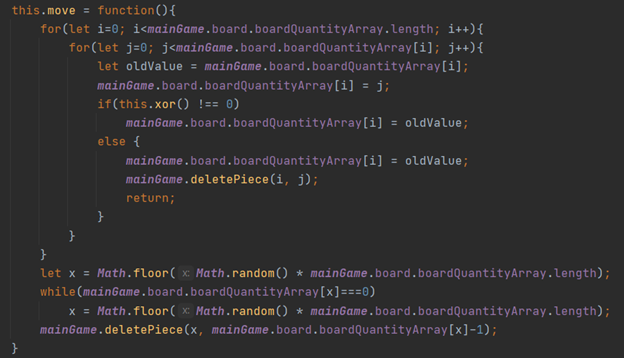
\includegraphics[width=14cm]{slike-kod/Slika11.png}
\caption{Prikaz određivanja novog poteza računala.}
\label{}
\end{figure}

\begin{figure}[H]
\centering
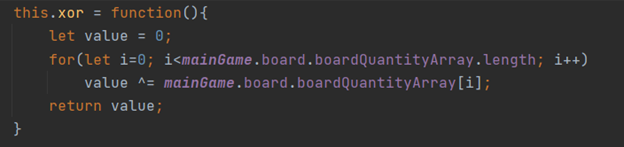
\includegraphics[width=14cm]{slike-kod/Slika12.png}
\caption{Prikaz funkcije xor().}
\label{}
\end{figure}





Pomoću funkcije Piece() stvara se nova loptica na ploči za igru. Kada je korisnik prešao mišem preko određenog broj loptica pomoću funkcije onmouseover označene loptice postaju bijele kako bi korisnik znao koje bi loptice uklonio eventualnim potezom. S druge strane, ako korisnik odustane od poteza, boja loptica ponovno postaje kakva je bila na početku bez uklanjanja. Tek klikom na lopticu korisnik uklanja loptice iz igre i čini svoj potez u igri, a loptice se tada brišu iz igre.


\begin{figure}[H]
\centering
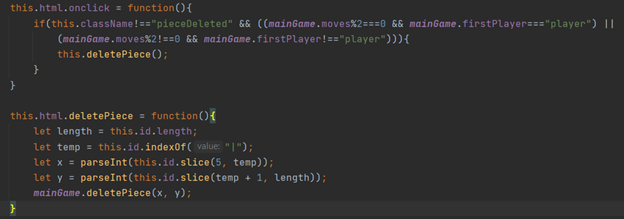
\includegraphics[width=14cm]{slike-kod/Slika13.png}
\caption{Prikaz funkcije za uklanjanje loptice iz igre.}
\label{}
\end{figure}